%{
\begin{octave}
  %}
  importLatest('kern')
  kernToolboxes
  % colordef white
  % randn('seed', 1e8)
  % rand('seed', 1e8)
  %{
\end{octave}
\begin{frame}[labels=skipGPProperties,fragile]
  \frametitle{Covariance for Transcription Model}
  {\textbf{RBF covariance function for $\tfConcentration\left(t\right)$}}
  \begin{center}
    \begin{align*}
      \only<1,3>{\mrnaConcentration_{i}\left(t\right)=\frac{\basalRate_{i}}{\decayRate_{i}}+\sensitivity_{i}\exp\left(-\decayRate_{i}t\right)\int_{0}^{t}\tfConcentration\left(u\right)\exp\left(\decayRate_{i}u\right)\text{d}u.}
      \only<2>{\mrnaConcentration &= \basalRate/\decayRate +\sum_i\mathbf{e}_i^\top\mathbf{\tfConcentration}\quad \mathbf{\tfConcentration} \sim \mathcal{N}\left(\mathbf{0},\Sigma_i\right)\rightarrow \mrnaConcentration \sim \mathcal{N}\left(\basalRate/\decayRate, \sum_i\mathbf{e}_i^\top\Sigma_i\mathbf{e}_i\right)}
  \end{align*}
\end{center}
  \begin{columns}[c]
    \column{4cm}
    \begin{itemize}
    \item Joint distribution for $\mrnaConcentration_{1}\left(t\right)$, $\mrnaConcentration_{2}\left(t\right)$, $\mrnaConcentration_{3}\left(t\right)$,
      and $\tfConcentration\left(t\right)$.

    \item Here:\vspace{0.1cm}
      {\tiny 
        \begin{tabular}{|c|c|c|c|c|c|}
          \hline 
          $\decayRate_{1}$ & $\sensitivity_{1}$ & $\decayRate_{2}$ & $\sensitivity_{2}$ & $\decayRate_3$ &  $\sensitivity_3$\\
          \hline
          \hline 
          5 & 5& 1 & 1& 0.5 & 0.5\\
          \hline
        \end{tabular}
      }
    \end{itemize}

    \column{8cm}

    \begin{center}
      \begin{octave}
        %}
        close all
        columnWidth = 8;
        numSamp = 100;
        t = linspace(0, 5, numSamp)';
        kern = kernCreate(t, {'multi', 'rbf', 'sim', 'sim', 'sim'});
        for i = 1:length(kern.comp)
          kern.comp{i}.inverseWidth = 1/(0.75*0.75);
        end
        kern.comp{2}.decay = 5;
        kern.comp{2}.variance = 25;
        kern.comp{3}.decay = 1;
        kern.comp{3}.variance = 1;
        kern.comp{4}.decay = 0.5;
        kern.comp{4}.variance = 0.25;
  
        params = kernExtractParam(kern);
        kern = kernExpandParam(kern, params);
  
        K = kernCompute(kern, t);
        imagesc(1:400, 1:400, K, [-1.1 1.1]);
        handle = [];
        handle = [handle; text(100, 430, '\small $\tfConcentration(t)$', 'horizontalalignment', 'center')];
        handle = [handle; text(200, 430, '\small $\mrnaConcentration_1(t)$', 'horizontalalignment', 'center')];
        handle = [handle; text(300, 430, '\small $\mrnaConcentration_2(t)$', 'horizontalalignment', 'center')];
        handle = [handle; text(400, 430, '\small $\mrnaConcentration_3(t)$', 'horizontalalignment', 'center')];
        set(handle, 'horizontalalignment', 'right')
        handle = [handle; text(-40, 50, '\small $\tfConcentration(t)$', 'horizontalalignment', 'center')];
        handle = [handle; text(-40, 150, '\small $\mrnaConcentration_1(t)$', 'horizontalalignment', 'center')];
        handle = [handle; text(-40, 250, '\small $\mrnaConcentration_2(t)$', 'horizontalalignment', 'center')];
        handle = [handle; text(-40, 350, '\small $\mrnaConcentration_3(t)$', 'horizontalalignment', 'center')];
        axis off
        %colorbar
        printLatexPlot('simKernImage', '../../../kern/tex/diagrams', 0.8*columnWidth) 
        %{
      \end{octave}
      \inputdiagram{../../../kern/tex/diagrams/simKernImage}
      %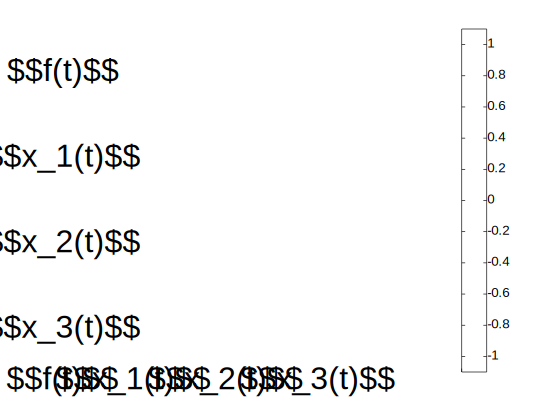
\includegraphics[width=0.8\columnwidth]{../../../kern/tex/diagrams/simTestKernelImage}
    \end{center}
  \end{columns}
\end{frame}
%}